\documentclass[a4paper,
fontsize=11pt,
%headings=small,
oneside,
numbers=noperiodatend,
parskip=half-,
bibliography=totoc,
final
]{scrartcl}

\usepackage[babel]{csquotes}
\usepackage{synttree}
\usepackage{graphicx}
\setkeys{Gin}{width=.4\textwidth} %default pics size

\graphicspath{{./plots/}}
\usepackage[ngerman]{babel}
\usepackage[T1]{fontenc}
%\usepackage{amsmath}
\usepackage[utf8x]{inputenc}
\usepackage [hyphens]{url}
\usepackage{booktabs} 
\usepackage[left=2.4cm,right=2.4cm,top=2.3cm,bottom=2cm,includeheadfoot]{geometry}
\usepackage{eurosym}
\usepackage{multirow}
\usepackage[ngerman]{varioref}
\setcapindent{1em}
\renewcommand{\labelitemi}{--}
\usepackage{paralist}
\usepackage{pdfpages}
\usepackage{lscape}
\usepackage{float}
\usepackage{acronym}
\usepackage{eurosym}
\usepackage{longtable,lscape}
\usepackage{mathpazo}
\usepackage[normalem]{ulem} %emphasize weiterhin kursiv
\usepackage[flushmargin,ragged]{footmisc} % left align footnote
\usepackage{ccicons} 
\setcapindent{0pt} % no indentation in captions

%%%% fancy LIBREAS URL color 
\usepackage{xcolor}
\definecolor{libreas}{RGB}{112,0,0}

\usepackage{listings}

\urlstyle{same}  % don't use monospace font for urls

\usepackage[fleqn]{amsmath}

%adjust fontsize for part

\usepackage{sectsty}
\partfont{\large}

%Das BibTeX-Zeichen mit \BibTeX setzen:
\def\symbol#1{\char #1\relax}
\def\bsl{{\tt\symbol{'134}}}
\def\BibTeX{{\rm B\kern-.05em{\sc i\kern-.025em b}\kern-.08em
    T\kern-.1667em\lower.7ex\hbox{E}\kern-.125emX}}

\usepackage{fancyhdr}
\fancyhf{}
\pagestyle{fancyplain}
\fancyhead[R]{\thepage}

% make sure bookmarks are created eventough sections are not numbered!
% uncommend if sections are numbered (bookmarks created by default)
\makeatletter
\renewcommand\@seccntformat[1]{}
\makeatother

% typo setup
\clubpenalty = 10000
\widowpenalty = 10000
\displaywidowpenalty = 10000

\usepackage{hyperxmp}
\usepackage[colorlinks, linkcolor=black,citecolor=black, urlcolor=libreas,
breaklinks= true,bookmarks=true,bookmarksopen=true]{hyperref}
\usepackage{breakurl}

%meta
%meta

\fancyhead[L]{Redaktion LIBREAS\\ %author
LIBREAS. Library Ideas, 39 (2021). % journal, issue, volume.
\href{http://nbn-resolving.de/}
{}} % urn 
% recommended use
%\href{http://nbn-resolving.de/}{\color{black}{urn:nbn:de...}}
\fancyhead[R]{\thepage} %page number
\fancyfoot[L] {\ccLogo \ccAttribution\ \href{https://creativecommons.org/licenses/by/4.0/}{\color{black}Creative Commons BY 4.0}}  %licence
\fancyfoot[R] {ISSN: 1860-7950}

\title{\LARGE{Editorial \#39: Roboter und Automatisierung}}% title
\author{Redaktion LIBREAS} % author

\setcounter{page}{1}

\hypersetup{%
      pdftitle={Editorial \#39: Roboter und Automatisierung},
      pdfauthor={Redaktion LIBREAS},
      pdfcopyright={CC BY 4.0 International},
      pdfsubject={LIBREAS. Library Ideas, 39 (2021).},
      pdfkeywords={Automatisierung, Roboter, Bibliothek},
      pdflicenseurl={https://creativecommons.org/licenses/by/4.0/},
      pdfcontacturl={http://libreas.eu},
      baseurl={http://libreas.eu},
      pdflang={de},
      pdfmetalang={de}
     }



\date{}
\begin{document}

\maketitle
\thispagestyle{fancyplain} 

%abstracts

%body
{\par \centering Wir widmen diese Ausgabe Christa Nowakowski (1946--2021).\par}

{\par \centering ***\par}

Wir haben aufgerufen zum 100-jährigen Jubiläum des Begriffs des
\enquote{Roboters}\footnote{Am 25. Januar 1921 hatte in Prag Karel
  Čapeks Theaterstück R.U.R. - Rossum's Universal Robots Premiere, siehe
  Karel Čapek, R.U.R. -- Rossum's Universal Robots, Aventinum: Prag
  1920.} Beiträge einzusenden und das Thema auf die fortschreitende
Technisierung und Automatisierung in Bibliotheken erweitert. Im Fokus
des Covers befindet sich eine Abwandlung aus dem Deckenfresko von
Michelangelos \enquote{Die Erschaffungs Adams}.\footnote{An dieser
  Stelle danken wir herzlich Samantha Tirtohusodo und Nora Marlene
  Diepenbrock, die im Sommersemester 2021 am Institut für Bibliotheks-
  und Informationswissenschaft am Projektseminar LIBREAS - Digitale
  Wissenschafts- und Fachkommunikation teilgenommen und das Cover
  entwickelt haben. Dazu beschreiben sie den Prozess der Gestaltung wie
  folgt:

  Der Mensch erschuf die Maschine. Die Lücke zwischen den Fingern, die
  im originalen Gemälde für die Distanz zwischen Göttlichkeit und
  Menschsein steht, wird auch auf dem Cover beibehalten, um die
  Abgrenzung zwischen Mensch und Maschine darzustellen. Der Verlauf
  zwischen Schrift und Binärcode, versetzt zu Roboter und Mensch,
  repräsentiert den aktuellen Konflikt zwischen analog und digital in
  Bibliotheken.}

Herausgekommen sind -- neben einem Text zum aktuellen Einsatz eines
Roboters an der Fachhochschule Nordwestschweiz (FHNW) -- eher historisch
ausgerichtete Texte zu den Themen Digitalisierung und Automatisierung in
(wissenschaftlichen) Bibliotheken sowie am Deutschen Museum in München.
Mit diesen Themen beschäftigen sich Bibliotheken schon lange, so sind
die historischen Ansätze in den Beiträgen nachvollziehbar. Vielleicht
sind vor allem die Automatisierung und Digitalisierung einfach bereits
Realität und nichts Neues mehr?

Auch Roboter werden bereits in einigen Bibliotheken, zum Teil seit
vielen Jahren, eingesetzt. Kritische Beiträge beispielsweise gegenüber
diesen anthromorphisierten Zeitgenoss*innen oder Artikel zu ethische
Bedenken oder Ängsten haben wir kaum erhalten. Überwiegt womöglich der
pragmatische Blick auf den Nutzen der Technisierung und die Freude über
die Massen-Digitalisierung und Automatisierung?

In Bibliotheken\footnote{Bereits 2016 sprach der ZBW Mediatalk-Blog von
  einem Revival der Chatbots in Bibliotheken, siehe
  \url{https://www.zbw-mediatalk.eu/de/2016/05/revival-der-chatbots-revolution-des-kundenkontakts-disruption-des-software-marktes/}}
und öffentlichen Behörden ist zudem eine Renaissance der Chatbots
feststellbar. Nahezu jedes deutsche Bundesland nutzt einen Chatbot für
die zahlreichen Anfragen zum Thema COVID-19: In Berlin gibt
beispielsweise ein Bär namens "Bobbi" mehr oder weniger
zufriedenstellend Auskunft zu gängigen Fragen wie "Darf man wieder
verreisen?"

\begin{figure}
\centering
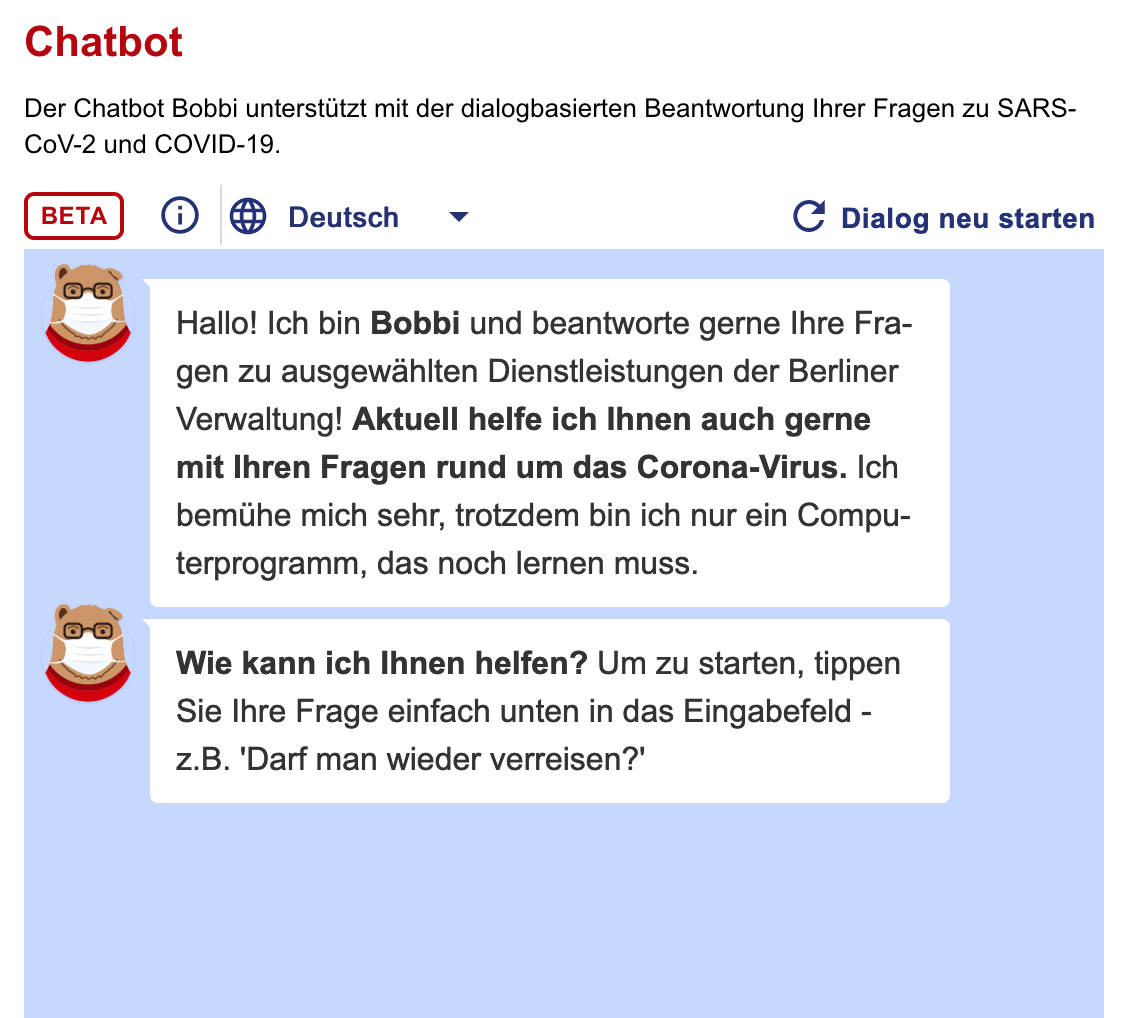
\includegraphics[width=.6\textwidth]{img/img1}
\caption{Der Regierende Bürgermeister von Berlin (2021): Senatskanzlei
Informationen zum Coronavirus (Covid-19), Chatbot Bobbi:
\url{https://www.berlin.de/corona/faq/chatbot/artikel.917495.php}}
\end{figure}

Ob durch diese automatisierte und auch distanzierte Form der
Kommunikation die Unsicherheiten und Ängste zu diesem Thema adäquat
aufgefangen werden können, ist zu bezweifeln.

Diese Ausgabe entstand wieder im virtuellen Raum, eingetaktet zwischen
zahlreichen anderen Webex-, Zoom-, Jitsi-, Discordterminen\footnote{Hier
  möchten wir ebenso Victoria Geske und Yannick Paulsen aus dem
  LIBREAS-Projektseminar danken, die uns einen wertvollen Einblick in
  das Communitybuilding mit Discord im DACH-Raum geben.} und digitalen
Konferenzen sowie in unseren privaten Wohnungen, die auch zugleich
unsere Arbeitsplätze sind, also in der Lebensrealität der Pandemie, die
nun seit über einem Jahr unser Leben bestimmt.

Umso erfreulicher ist, dass sich trotz der besonderen Umstände mit Sara
Juen eine neue Kollegin für die Mitarbeit in der Redaktion gewinnen
ließ. Wir heißen sie herzlich willkommen.

Wir wünschen Ihnen und euch weiterhin viel Kraft, Durchhaltevermögen und
vor allem Gesundheit!

***

Die LIBREAS. Library Ideas

Eure / Ihre Redaktion LIBREAS. Libreas

(Berlin, Hannover, Göttingen, Lausanne, München)

\begin{figure}[t]
\centering
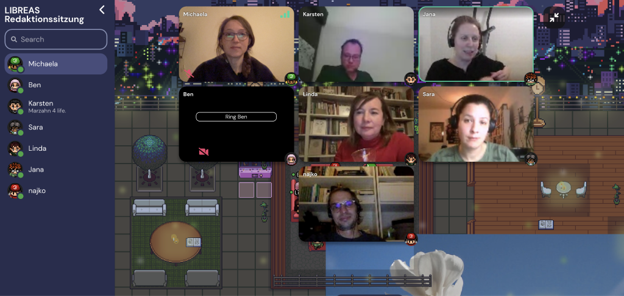
\includegraphics[width=.9\textwidth]{img/img2}
\caption{Redaktionsorte - Immer noch online}
\end{figure}

\end{document}
